\chapter{Research Design}
\label{resdes}

\begin{figure}[h]
	\centering
	\captionsetup{justification=centering}
\scalebox{.40}{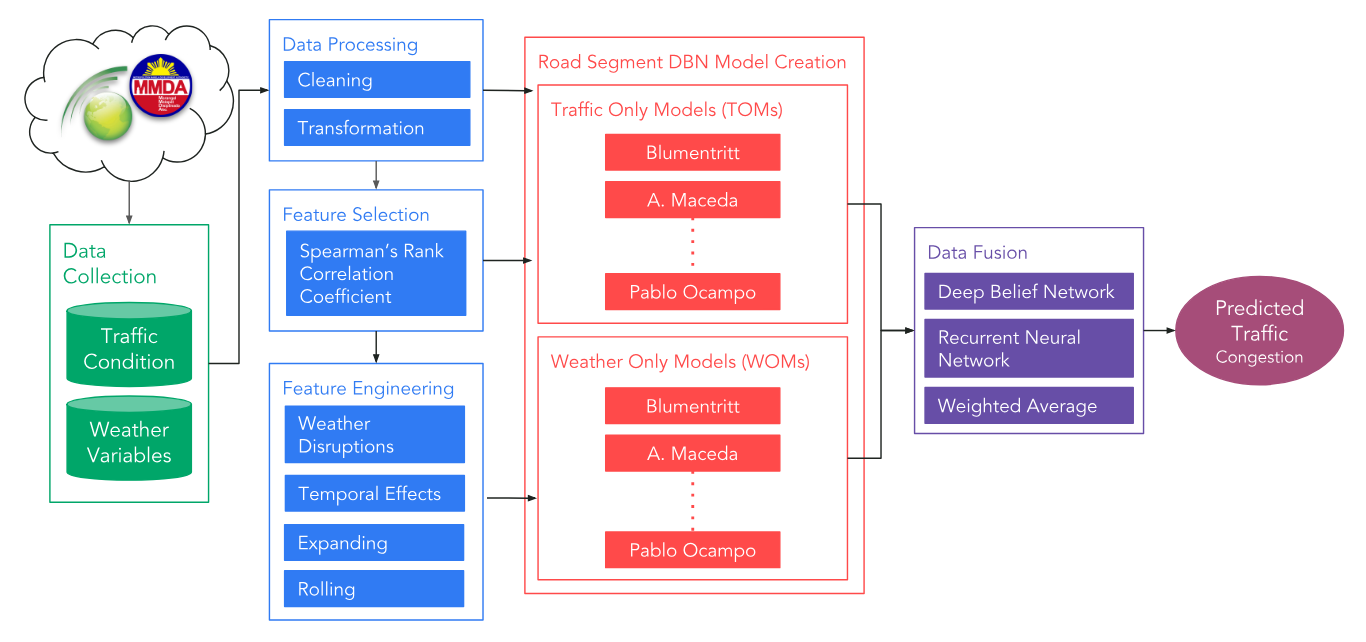
\includegraphics{THESIS_ResearchDesignFinal.png}}
	\caption{Research Framework}
	\label{fig:framework}
\end{figure}

Figure \ref{fig:framework} illustrates the whole framework for the research. First, this research collected historical traffic condition from MMDA and historical weather variables from WWO. These raw data were cleaned and re-sampled to match the time intervals of the data using linear interpolation and was transformed to their normalized values. The data was explored and analyzed to identify seasonality and trends present for both traffic and weather. Analyses and insights collected were used to select and engineer features to use in the model to predict traffic. These features include rolling and expanding window features, which are in-depth statistical features of traffic such as the mean, minimum, and maximum values of past traffic of a certain time period.

The final variables and engineered features were fed into the Traffic-Only Models (TOM) and Weather-Only Models (WOM), which were developed in DBN, for the 14 road segments in Manila for both wet and dry season. Additionally, analyses were evaluated through the training of the models. Two different fusion levels were tested in this model, specifically at the feature level and at the decision level. For the decision level, three fusion techniques were tested, particularly DBN, RNN, and WA. The model was evaluated using RMSE and MAE. The model’s sensitivity was also explored to analyze the relevance of input variables. 



\section{Data Collection}
\label{rd_datacollection}
There were two public datasets collected: one for traffic and one for weather. The traffic dataset was obtained from Metro Manila Development Authority (MMDA) traffic monitoring system, while the weather dataset was collected from World Weather Online (WWO). Both datasets were collected from January 2015 to December 2015.

\subsection{Traffic Dataset}
There were two limitations found from the traffic dataset. First is that the traffic conditions were only represented as \textit{light} (L), \textit{moderately light} (ML), \textit{moderate} (M), \textit{moderately heavy} (MH), and \textit{heavy} (H). Since this dataset only had five values to classify the traffic condition in a particular road segment, this might cause underfitting in our model since it was used as input for a regression problem. Moreover, it could also contribute to poor correlation as these five values were correlated with continuous weather variable values. Instead, they were converted to their equivalent estimated traffic speed provided by the MMDA (see Table \ref{table_traffic_condition}). These speeds are further converted to congestion intensity, represented as their reciprocal so that the data would be easier to interpret such that higher value means higher congestion level.


\begin{table}[h]
\centering
\caption{Traffic speed equivalent of traffic conditions}
\label{table_traffic_condition}
\begin{tabular}{|l|r|}
\hline
\textbf{Traffic Condition} & \multicolumn{1}{l|}{\textbf{Equivalent Speed (kph)}} \\ \hline
Light (L) & 36 - 60 \\ \hline
Moderately Light (ML) & 31 - 35 \\ \hline
Moderate (M) & 16 - 30 \\ \hline
Moderately Heavy (MH) & 11 - 15 \\ \hline
Heavy (H) & 0 - 10 \\ \hline
\end{tabular}
\end{table}

Another limitation was that the traffic dataset contains missing records. Out of 935,200 records, there were 93 rows wherein the traffic condition of that road segment in that particular time interval was not recorded as indicated by \textit{none} (N) condition. Furthermore, having only 935,200 records from a sample from 2015, having a 15-minute interval for 14 road segments, meant that 45,920 records were missing as well. This implied that inconsistencies may occur as the missing data would need to be filled to make the data continuous. To do this, those missing values were replaced through linear interpolation. 
Apart from the limitations, there were other factors considered in this study. Since this study is only concerned road segments from Manila, only the road segments under it were used. As a result, 14 out of 142 road segments were only considered: 7 roads from Roxas Boulevard and 7 roads from España.

\subsection{Weather Data}
The collected weather dataset from WWO featured a complete hourly reading of the weather variables for Manila. One downside of this dataset, however, was that the weather data generalizes the weather for the whole city. This implied inconsistencies when correlating the traffic condition to the weather variables as the weather at one road is not the same as the weather of another, despite being in the same city.

Additionally, the hourly weather dataset needed to be matched with the 15-minute interval of the traffic dataset. This was done by resampling and linear interpolating the dataset to have a 15-minute time interval.

\section{Pattern Analysis}
To be able to determine the relationship of weather to traffic, it is important to understand the underlying pattern between these two datasets. In the following analyses, traffic will be treated as the dependent variable and weather as the independent variable. These are approached in four steps. First, patterns of traffic with itself are analyzed by its seasonality and daily trend. Second, weather is analyzed with respect to traffic, likewise, in terms of seasonality and daily trend. With the relationship of weather and traffic identified, weather disruptions are characterized and identified as a prerequisite for the next step. As weather disruptions are determined, disruptions on the normal traffic pattern could be identified.

\subsection{Traffic Analysis}
Before understanding the effects of weather to traffic, it is necessary to understand the underlying pattern of traffic as it may have its own existing pattern that might neglect the effects of weather. On an average day, traffic could be linked with the people's daily transportation demand. One example of these is the daily commute of people, attributed to their organizational duties (i.e. 9 to 5 jobs) and academical duties. Built upon these expected demands, traffic could be expected to be daily seasonal on working days. Given this statement, to understand traffic, two terms must be understood: seasonality and working days.

Seasonality refers to a predictable pattern of a time series data that regularly repeats after a number of intervals. To identify the seasonality of a variable, the similarity between an observation and time lags between them were analyzed through autocorrelation. \textit{Lags} refer to the time delay of one observation on another. For instance, the delay between the traffic observations at June 18 and June 19 is indicated by a one-day lag.

Understanding seasonality is significant to determine the duration of a certain pattern which could be used as a guide in predicting an incoming observation. In terms of traffic, it is known to be seasonal with its previous day (e.g. Tuesday with Monday) and its previous week (e.g. Monday with the previous Monday) \shortcite{kumar2015short}.

Traffic's \textbf{previous day} seasonality could be perceived as causal, such that the traffic of yesterday could be attributed to the traffic of today. For instance, having an intense traffic yesterday morning could be linked with the incoming morning traffic of today. In inheriting the factors of previous days, nonetheless, we also need to take into consideration the concept of working and non-working day.

A \textit{working day} refers to a day in which people are assigned on duty in an organization \cite{liu2008wdcm}. For most organizations, it is defined to be on weekdays, Mondays to Fridays, while non-working days are on weekends, Saturdays to Sundays. Aside from weekends, though, non-working days also occur during holidays and government-announced class/work suspension. In the following analyses, those days are treated as outliers to our data as the traffic pattern for that particular day is irregular compared with the other weekday working day records. These are important to consider as the transportation demand during working days are higher compared with non-working days \cite{traffic_trend}. For example, the transportation demand of Monday is significantly different from Sunday, thus referencing Sunday for the expected pattern of Monday would be erroneous.

With the difference of the transportation demand during working days and non-working days, the concept of peak hour must also be considered \shortcite{de2008traffic}. Peak hour refers to the busiest hour where traffic is expected to rapidly rise \shortcite{downs1962law}. In the case of Metro Manila, peak hours are expected to occur from 7 AM to 10 AM, when people leave their home to go to their respective organizations, and 4 PM to 7 PM, when they depart their organizations and return home \shortcite{metro_manila_peak_hour}.

On the other hand, traffic’s \textbf{previous week} seasonality could be perceived as occasional. Monday \shortcite{rakha1995statistical} and Friday \shortcite{datla2008impact} traffic could be observed as more congested as compared with the other weekday traffic. Unlike previous day traffic, it does not matter if it is a working day or a non-working day as Mondays are based on the pattern of previous Mondays. The advantage of this, in fact, is that traffic is no longer causal, thus a normal pattern could be derived using its pattern from the succeeding weeks.



\subsection{Weather Analysis}
With the pattern of traffic taken into consideration, the relationship between weather and traffic could now be better understood. To have an overview of the relationship between traffic and weather variables, Spearman’s rank correlation is performed to measure the non-linear relationship between these two. Although given that traffic has its own pattern and weather generally has a one-way relationship with traffic, it is expected for these two to not have a direct relationship \shortcite{tanner1952effect}.

To verify this, an exploratory analysis was performed by examining the commonalities of traffic and each weather variables through its seasonality and trend. From this, a normal trend will be defined based on their average per time interval on a given common seasonality. Then, a more specific relationship could be defined by relating their trends.

\subsection{Weather Disruption}
With the general relationship between traffic and weather examined, the effects of weather on traffic could now be assessed. These are primarily focused on rainfall potentially disrupting the normal trend of traffic. To identify these, climate seasonality is classified, and rainy weather conditions are utilized.

The classification of seasons is significant to determine the months when precipitation is rampant. This is measured by getting the average of precipitation on a given month. In conjunction, rainy weather conditions may also provide a more general insight with regards to the rainfall intensity at a given time period. These are classified into 11 conditions: patchy rain possible, patchy light rain, light rain, light rain shower, light rain, moderate rain at times, moderate rain, moderate or heavy rain shower, heavy rain at times, heavy rain and torrential rain showers.


\subsection{Traffic Disruption}
As weather disruption dates are identified, verification whether rainfall really does affect traffic could be performed. As mentioned in the earlier analysis of traffic seasonality, traffic is said to be daily seasonal and weekly seasonal. Since it is expected that rainfall may potentially disrupt the normal trend of traffic, then it is expected that this seasonality would be affected. In general, this is examined by comparing the seasonality of traffic between different climate seasons through autocorrelation. 

\section{Correlation Analysis}
\subsection{Correlation of Engineered Traffic Features with Traffic Condition}

Given the initial seasonality analysis and findings on how different a disrupted traffic pattern is compared to its normal pattern, a potential weakness of using one instance of its seasonal day alone is that it may be a disrupted pattern, hence it would not be a reliable guide for the incoming traffic. With that in mind, more reliable features are engineered with the aim of minimizing the identified weakness.

To address this problem, a concept of normal pattern for a given day must be defined. One way to approach this is by getting the average traffic per time interval from a number of instances of seasonal days. For instance, having the mean of one disrupted day and one normal day is a better basis than one disrupted day. Scaling up the range, getting the mean of a number of normal days with the inclusion of one disrupted day can override the effects of the single disruption.


\subsection{Correlation of Immediate Traffic Features with Traffic Condition}
Lastly, the relationship between the engineered traffic features to the current traffic feature was explored. Before exploring this relationship, traffic features were engineered from the current traffic feature in order to give information of the immediate past traffic, and its relationship with the current traffic. These engineered traffic features include rolling and expanding window features, statistical description of past time period such as the mean traffic six weeks ago, and flags for significant traffic patterns such as the work day and peak hours. Exploring the relationship between these engineered traffic features with the current traffic feature also give a better representation of the effect of disruptions present in the immediate past to the current traffic.

As mentioned, rolling and expanding window features were engineered to represent the immediate past traffic. Rolling and expanding traffic features were generated for window sizes \textit{4, 8, 24, 48}, and \textit{96}, with each window representing a 15-minute time interval. Thereby, the generated window sizes translates to \textit{1, 2, 6, 12}, and \textit{24}-hours time interval. The statistical features such as the mean, minimum, and maximum for both rolling and expanding windows were generated to describe the immediate past traffic conditions given a specific window size.


\subsection{Correlation between Connected Road Segments}
There are a number of factors contributing to traffic. For instance, given a point-to-point road segment, traffic in one road segment could be due to its connected road segment carrying over its traffic. As the road segments in the utilized dataset are just samples from a larger road network, a road segment may be skipped through their connected intersections. With road segments analyzed with their own pattern, the next step is to analyze them as part of a whole road.

Identifying the relationship between connected road segments are significant as it allows a certain road to have a generalized description based on their common characteristics. Furthermore, this is necessary as this relationship defines if the effect of weather on one road segment is the same with its neighboring road segments. To verify this, given that these road segments have a matching seasonality, the average of their traffic per time interval based on their seasonality could be evaluated. Then, their correlation could be evaluated by using Pearson correlation coefficient to analyze their linear relationship.




%TRAFFIC MODEL CREATION
\section{Model Implementation}
Features were engineered in order to represent the immediate past traffic, and other trends and patterns of traffic. Additionally, weather features were selected through correlation analysis. These features are as follows:

\begin{enumerate}
\item Temporal Information of the respective traffic record represented as Month, Day, Hour, Minute, Day of Week,
\item Traffic a Day before represented as L, ML, M, MH, H
\item Traffic 6 weeks ago represented as L, ML, M, MH, H
\item Current Traffic represented as L, ML, M, MH, H
\item Rolling and Expanding Traffic Features (mean, max, and minimum) for windows 4, 8, 24, 48, and 96 represented as L, ML, M, MH, H,
\item Weather Variables (wind speed, wind gust, temperature, humidity, dew point, precipitation, visibility, pressure, cloud cover, heat index, and feels-like) represented in their respective measurements
\end{enumerate}

A model implemented using Deep Belief Network (DBN) used these features that represent the past traffic to predict the current traffic condition intensity.

\subsection{Prediction Models}
According to the framework in \ref{fig:framework}, two models were implemented using Deep Belief Network (DBN): the Traffic-Only Model (TOM) and the Weather-Only Model (WOM). The TOM considers historical traffic condition intensity to predict traffic, while the WOM only considers historical weather variables to predict traffic. In this study, these DBN models were implemented with the open source machine learning framework in Python, \textit{tensorflow}. The TOM and WOM network architectures are shown in \ref{tab:dbn_models_architecture}. 

\begin{table}[h]
\centering
\caption{DBN Models Network Architecture}
\label{tab:dbn_models_architecture}
\begin{tabular}{|l|l|l|c|l|l|}
\hline
                 & \textbf{\begin{tabular}[c]{@{}l@{}}Pre-Train \\ Epochs\end{tabular}} & \textbf{\begin{tabular}[c]{@{}l@{}}Fine-Tune\\ Epochs\end{tabular}} & \multicolumn{1}{l|}{\textbf{\begin{tabular}[c]{@{}l@{}}Activation\\ Function\end{tabular}}} & \textbf{\begin{tabular}[c]{@{}l@{}}Batch\\ Size\end{tabular}} & \textbf{\begin{tabular}[c]{@{}l@{}}Hidden Layer\\ Structure\end{tabular}} \\ \hline
\textbf{TOM}     & 7                                                                    & 80                                                                  & \multirow{4}{*}{relu}                                                                       & 192                                                           & {[}14, 375{]}                                                             \\ \cline{1-3} \cline{5-6} 
\textbf{WOM}     & 5                                                                    & 88                                                                  &                                                                                             & 96                                                            & {[}20, 85, 170{]}                                                         \\ \cline{1-3} \cline{5-6} 
\textbf{FEI-DEO} & 7                                                                    & 80                                                                  &                                                                                             & 192                                                           & {[}14, 375{]}                                                             \\ \cline{1-3} \cline{5-6} 
\textbf{DEI-DEO} & 8                                                                    & 350                                                                 &                                                                                             & 192                                                           & {[}20, 50, 100{]}                                                         \\ \hline
\end{tabular}
\end{table}


% For the TOM, there are two hidden layers with 14 and 375 units respectively. The TOM was trained with 11 epochs during the pre-training phase, and 80 epochs during the fine-tuning phase. For the WOM, there are 3 hidden layers with 14, 85, and 170 units respectively. The WOM was trained with 5 epochs during the pre-training phase, and 88 epoch during the fine-tuning phase. The learning rate for both models DBN is 0.01 and RBM is 0.0. The activation function for both models is the $relu$ function.

DBNs are made up of stacks of Restricted Boltzmann Machines (RBM). The training for DBN consists of two phases: pre-training and fine-tuning. In pre-training, each RBM is trained individually, and the weights and biases of layers are fixed. In fine-tuning, the weights and biases of the whole network are updated via back propagation using labeled input data.

Figure \ref{fig:dbntraining} shows the process of how the TOM and the WOM using DBN was trained for prediction. The training process consists of three phases. In the first phase, the stacks of RBM (sRBM) within the network are trained individually. At the end of this phase, the weights and biases of the whole DBN are initialized. In the second phase, the DBN fine-tunes the initialized weights and biases using the backpropagation algorithm. The network after stage 2 is the trained and enhanced DBN. In the third phase, the network predicts the future traffic condition using a testing dataset.

\begin{figure}[h]
	\centering
	\captionsetup{justification=centering}
	\scalebox{.8}{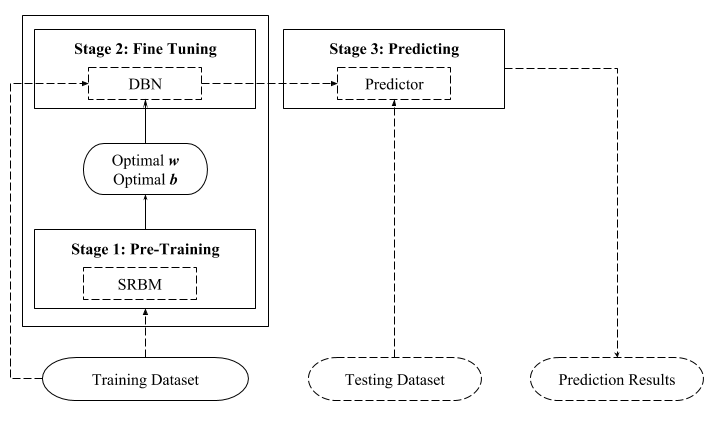
\includegraphics{dbntraining.png}}
	\caption{Structure of DBN Training Process}
	\label{fig:dbntraining}
\end{figure}

For the pre-training phase, the sRBM performs a number of forward and backward passes until the reconstructed data is close to the original input. The process of backward and forward passes is performed using the equations \ref{eq:4} and \ref{eq:5} to compute for the conditional probability of the hidden unit $h_j$ and visible unit $v_i$, respectively.

%Fine Tuning
For the fine-tuning phase, the loss function and activation function is defined.
The loss function for the softmax layer to improve the learning rate uses the cross-entropy equation between the visible and hidden units. The cross-entropy function is defined as
\begin{equation}
C = -\frac{1}{n}\sum_x [y ln a + (1 - y) ln (1-a)]
\end{equation}
\noindent where $n$ is the size of the training data, $x$ is the training input, $y$ is the desired output, and $a$ is the unit’s output.
For the activation function in the fine-tuning phase, the rectifier function was used for its nonlinearity activation capability. The rectifier function is defined as
\begin{equation}
f(x) = x^+ = max(0, x)
\end{equation}


\subsection{Data Fusion Model}
Data fusion is significant to see the effectiveness of adding weather as a factor in predicting traffic. This study evaluated two fusion approaches: Feature In-Decision Out (FEI-DEO) and Decision In-Decision-Out (DEI-DEO). In the FEI-DEO approach, traffic and weather features are fused in one dataset first before being used by the model to predict traffic. The DEI-DEO approach, meanwhile, predicts traffic through TOM and WOM, and fuses the prediction of both models into one final prediction. DBN is used in the FEI-DEO approach, while three algorithms are tested in the DEI-DEO approach which are Weighted Average (WA), Recurrent Neural Network (RNN) and DBN. 



%WEIGHTED AVERAGE
\subsubsection{Weighted Average}
The weighted average data fusion method used the predicted traffic from TOM and WOM. Both predictions were multiplied with its corresponding weight. Each weight was assigned based on the importance of the variable considered while keeping in mind the sum of the weights should be equal to 1. Then, the mean of the weighted predictions of both TOM and WOM will be calculated. The result will be the fused final traffic prediction.



%NEURAL NETWORK
\subsubsection{Neural Network}
The fusion model was also developed in two neural networks: Recurrent Neural Network (RNN) and Deep Belief Network (DBN) in evaluating DEI-DEO fusion approach. Only DBN was implemented in evaluating FEI-DEO approach.

In FEI-DEO, the traffic congestion intensity and weather variables were fused into one dataset before feeding it into the prediction model. The network will be trained to predict the traffic condition based on both traffic and weather in one model for the current time period $t$. The training of the network will continuously adjust weights and biases from comparing the generated output with the actual traffic condition. 

% The DBN for FEI-DEO fusion has 1 input layer, 3 hidden layers, and 1 output layer. There are 5 epochs for the pre-training phase, and 150 epochs for the fine-tuning phase. The learning rate for both DBN and RBM is 0.01.

In DEI-DEO, the traffic congestion intensity was predicted first with two prediction models, TOM and WOM. The prediction of these two prediction models was used into another model that will fuse the two predictions into one improved final prediction. The network will be trained to predict the traffic congestion intensity for the current time period $t$ through backpropagation by comparing the generated traffic condition prediction to the expected prediction, and adjusting the weights and biases of units and layers to fuse the two decisions to arrive at a prediction close to the expected. The input layer will have the predicted traffic condition of TOM and WOM.

The DBN model network archicture for both FEI-DEO and DEI-DEO fusion are also shown in \ref{tab:dbn_models_architecture}. The RNN for DEI-DEO fusion have only have 1 input layer, 1 hidden layer, and 1 output layer. The number of units for the hidden layer of the RNN will be determined through trial and testing starting from 5 to 100 units.

%TRAINING
\section{Training}
The collected dataset for traffic and weather was divided into two subsets; wet and dry season. The wet season dataset consists of data from the months of May to October 2015, while the dry season dataset consists of data from the months of November to April 2015. The models were tested on these datasets to evaluate the inclusion of weather variables.

Datasets were split into training and testing datasets. The training dataset was used during the pre-training and fine-tuning of the model. In the fine-tuning phase of the training of the model, the training dataset was labeled with the expected output so as to verify and adjust the weights and biases back from the pre-training. The label consists of the expected traffic condition given the input data. All data fed into the network are already normalized.

The training dataset for both prediction models TOM and WOM consists of data from the months of May to August was used for evaluating wet season, and months of January to April was used for evaluating the dry season. In turn, the testing dataset made use of the remaining months of the season: September to October for the wet season, and November to December for the dry season.

\subsection{TOM Training Dataset}
Training datasets for TOM include traffic features in a 15-minute time interval that were derived from insights in the exploratory data analysis. These traffic features include the following:
 \begin{enumerate}
\item Temporal information of the respective time period (i.e. month, hour, minute, day, and day of week);
\item Traffic condition intensity a day before the respective traffic;
\item Flags on working day and peak hour of the respective time period;
\item Rolling and expanding window features (which consist of the minimum, maximum, and mean for each window) for the immediate past traffic of the respective traffic; and
\item Average traffic 2 weeks before the respective traffic.
\end{enumerate}

Different combinations of these traffic features are generated as separate training datasets to compare the performance of the model with the respective feature combination. These feature combinations are denoted as the following: 

\begin{enumerate}
\item \textit{OT} - Features that only consist of the past traffic a day before the current;
\item \textit{OTWP} - Features including past traffic a day before the current, and flags on the workday and peak hour, and;
\item \textit{WPRE}- Features including OTWP, plus the addition of rolling and expanding features of the traffic 15 minute in the past of the current. In subsequent discussions, any number following this notion pertains to the window size of both the rolling and expanding features (e.g. WPRE 4 pertains to the features that include rolling and expanding features of window size 4).
\end{enumerate}

The label for the training dataset consists of actual the 15-minute time interval of the traffic condition intensity of the respective time of the bound of the road segment to be predicted. For visualization purposes, the input including the labels is illustrated in Figure \ref{fig:TOM_TrainingTestingInput}


\begin{figure}
\centering
\captionsetup{justification=centering}
\scalebox{.70}{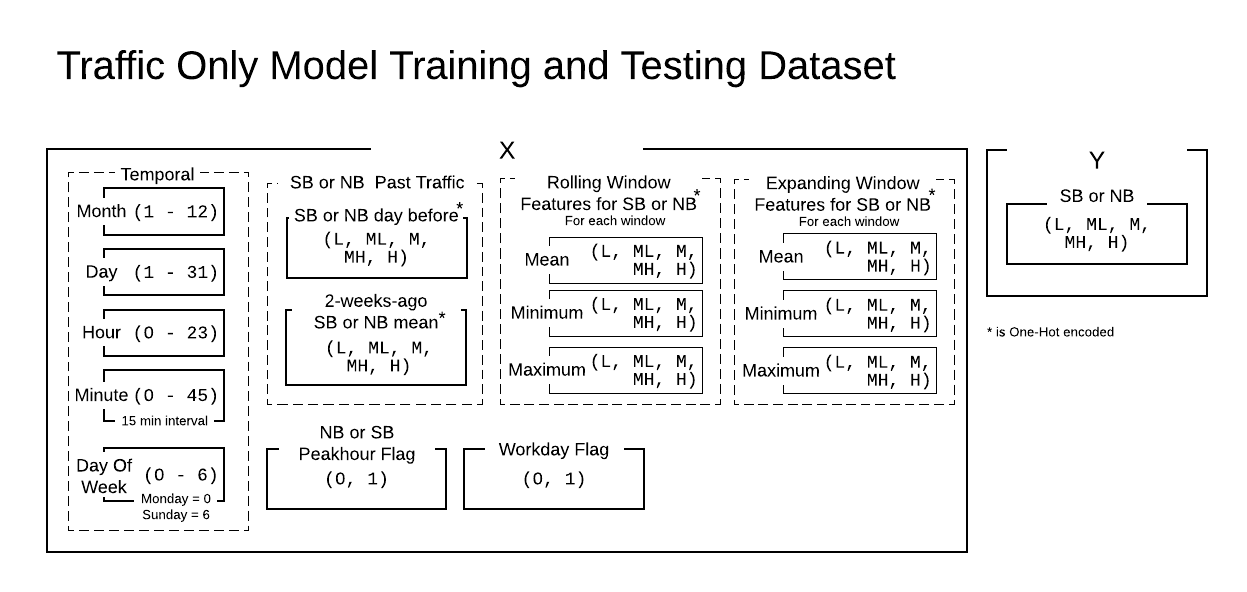
\includegraphics{TOM_TrainingTestingInput.png}}
\caption{A summary on the contents of the Traffic Only Model Training and Testing Dataset}
\label{fig:TOM_TrainingTestingInput}
\end{figure}

\subsection{WOM Training Dataset}
Training datasets for WOM include weather features in a 15-minute time interval that were derived and selected from insights in the exploratory data analysis. These weather features include the following:
\begin{enumerate}
\item Temporal Information of the respective time period (i.e. month, hour, minute, day, and day of week); and
\item Current weather variables (e.g. temperature, precipitation, wind speed, etc.) of the respective time period.
\end{enumerate}

Different combinations of these weather features are generated as separate training datasets to compare the performance of the model with the respective feature combination. These feature combinations are denoted as the following: 
\begin{enumerate}
\item Original Weather (OW) - all weather variables
\item All Correlated Weather (ACW) - all weather variables that have correlation between 0.1 to 0.3
\item Correlated Weather (CW) - all correlated weather variables excluding the redundant ones
\end{enumerate}

The label for the training dataset consists of the actual 15-minute time interval of the traffic condition intensity of the respective time of the bound of the road segment to be predicted.

\subsection{Fusion Model Training Dataset}
For the FEI-DEO model, the training dataset consists of merged training dataset used in the TOM and the WOM. The months for the training and testing datasets for this fusion model is also the same.

For the DEI-DEO model, the training dataset consists of the predicted traffic generated by TOM and WOM. The months for the training consists of the months of May to September for the wet season and January to April and November to December for the dry season. The testing dataset consists of the predicted traffic for the month of October and December. The label for the training dataset will consist of the 15-minute time interval of the actual traffic condition intensity of the respective time of the bound of the road segment to be predicted.

\section{Evaluation}

\subsection{Prediction Model Evaluation}
The performance of all models and algorithms (DBN, RNN, and WA) were evaluated using RMSE and MAE. To evaluate TOM and WOM, the performance of the TOM and the WOM with different feature combinations are compared with each other to see which input variables are needed in predicting the traffic condition intensity for the current time period $t$. The performance of the fusion models in the feature level (FEI-DEO) and in the decision level (DEI-DEO) was also evaluated. In evaluating DEI-DEO, the performance of the TOM and the WOM were initially evaluated before the fusion model/s. Then, three fusion techniques, namely WA, RNN, and DBN, were compared and evaluated to see the accuracy of the final prediction. In evaluating FEI-DEO, feature combinations used in evaluating TOM and WOM were used in the model. Additionally, the performance of the TOM and the final prediction of the DEI-DEO and FEI-DEO fusion models were evaluated to see the relevance of the inclusion of weather variables as a factor in predicting traffic.

\subsection{Sensitivity Analysis}
The model’s sensitivity was also explored to analyze the relevance of input variables. Sensitivity analysis is also performed to achieve higher accuracy through calibration of hyperparameters. Specifically, the sensitivity for the models TOM, WOM and DEI-DEO and FEI-DEO fusion center in DBN were evaluated. Different combinations of input variables were evaluated to see how much the inclusion and removal of a variable affect the final prediction. 
% The parameters of the network were also experimented with, specifically the number of hidden layers and its units, the number of epochs for pre-training, the fine-tuning, and the batch size.

First, the sensitivity of the models with changing input variables was evaluated. The different input variables were removed per experiment to see the effect of its inclusion. The combination of input variables was done in the feature combination in earlier evaluations of the model (e.g. OTWP, OT, WPRE, OW, etc). For example, variables of the OTWP feature combination were tinkered. Then, the variables of OT combination were evaluated, and so on. The base model, with all the features including temporal and past traffic, as compared with the model with the removed variables (with or without temporal information or past traffic), and its change in performance was evaluated. The changes in performance describe the sensitivity of the model. Change in performance is calculated by getting the difference between the base and new input, and dividing with the base input. Formula in performance change is defined as
\begin{equation}
C = \frac{x_{base} - x_{new}}{x_{base}}
\end{equation}

In evaluating TOM, two sets of test-cases were considered, (1) the effect of temporal information in consideration of traffic features, and (2) the effect of past traffic with and without the consideration of temporal information. The first test-case removes temporal information one-by-one, testing the performance of the model with only the selected temporal information, and traffic features. This traffic features include working day and peak hour flags, and rolling and expanding features, and mean traffic 6 weeks before, and traffic a day before. The second test-case removes traffic features one-by-one without or without temporal information. 

Much like TOM, two sets of test-cases were considered in evaluating WOM, (1) the effect of temporal information in consideration of weather features, and (2) the effect of each weather features with and without the consideration of temporal information. The first case is similar to TOM's first case. Instead of traffic features, weather features were experimented with. The second case removes weather features one-by-one, and compares other combination of weather features (i.e. all weather variables, all correlated weather variables with redundant variables, correlated weather variables without redundant variables).

